\clearpage
\section{Data Collection and Processing}

Data collection for this research was initially done using a sensor box connected with a webcam. Specifically, an AutoPi \cite{AutoPi} was connected with the OBD-2 port of the vehicle. Through this port, the AutoPi is able to all kinds of vehicle data such as RPM, speed, engine temperature etc. It depends on the specific vehicle which data sources are available. Additionally, the AutoPi is equipped with an accelerometer and GPS sensor. The OBD-2 connector is mandatory in all cars since 2004 in the EU\cite{EU1998} , and therefore it seemed like a reliable approach to collect data. With this method, XXX trips were collected. Unfortunately, there were two problems with this collection setup. First, the used webcam was unable to accurately record visual data due variable lighting changes. Initially, this was solved by recording visual data with an external smartphone. However, the second issue was more problematic. For this research we want to fuse visual and accelerometer data. However, the accelerometer data from the AutoPi was only sampled at a relative low frequency of 12.5 Hz. Further data processing operations would be problematic at such low sampling frequency.

Since the visual data was already collected with a smartphone. It was decided to also collect accelerometer and GPS data with that same smartphone. Specifically that smartphone is an Apple iPhone 12 Mini. The phone is located in a generic used phone holder attached to the windshield, see figure \ref{fig:smartphone-collector}. To  collect the data an open-source app was modified and deployed on the smartphone.\footnote{See \cite{ios_logger} for modified fork and \cite{ios_logger_original} for original. Main modification is to keep the smartphone from sleeping while collecting data.} With this app, the following data is collected:
\begin{itemize}
\item Visual data: recorded in 1280 x 720 at 30 frames per second. Each frame contain a specific timestamp when that frame was collected.
\item Accelerometer data: sampled at 100 Hz. 
\item Location data: sampled at 1 Hz. Contains GPS coordinates, but also travel heading and traveling speed.
\end{itemize}


\begin{figure}[H]
\begin{center}
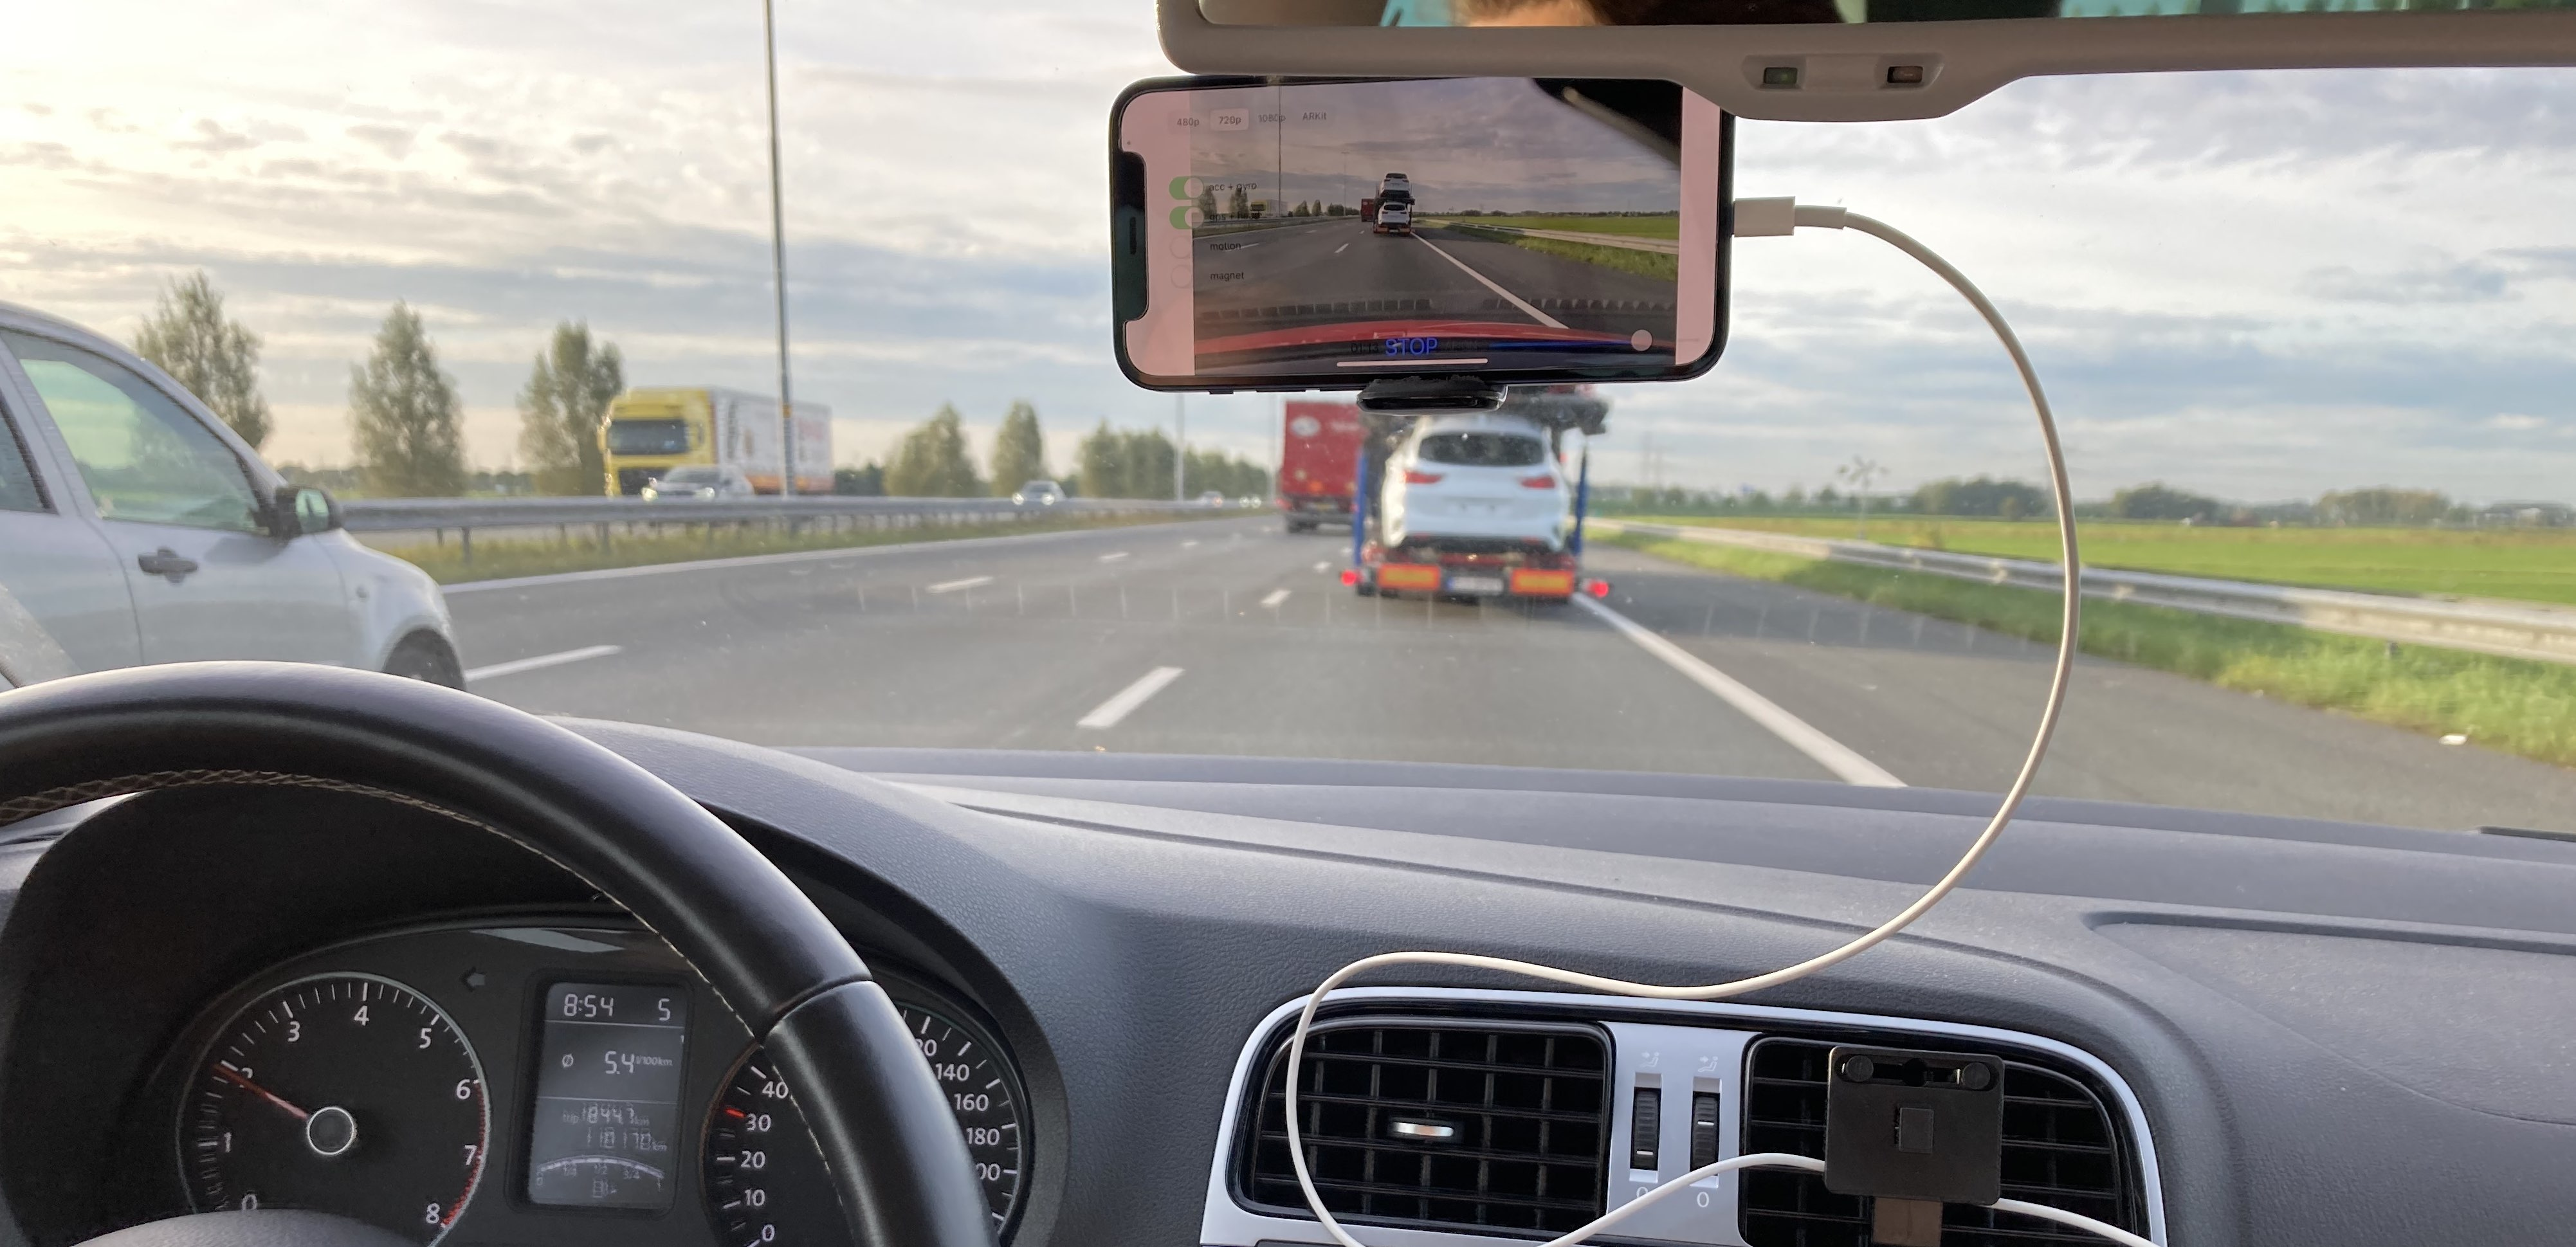
\includegraphics[width=\textwidth,keepaspectratio]{images/4_data/smartphone-setup.jpg}
\end{center}
\caption{Setup of smartphone to collect data.}
\label{fig:smartphone-collector}
\end{figure}

Data collected from the first approach is kept and visual data is still used to label visual objects. The processing steps for other sensor data (GPS and accelerometer) from the AutoPi and smartphone are equal. However, when noting sensor specifics, the latter collecting approach is assumed unless otherwise stated.


\subsection{Data Platform Architecture}
Currently AssetWorx lacks the infrastructure and architecture to process the collected data. In order to systematically process the collected data various data pipelines are designed. These pipelines can be holistically viewed as as a \textit{data platform architecture}. Implementation and execution of this platform is done on Google Cloud Platform (GCP) by using certain services GCP provides i.e. Kuberenetes and BigQuery. To orchestrate the various steps, Prefect\cite{Prefect} is used. Prefect is a dataflow automation tool. Although it is capable to orchestrate large scale workflows for data processing, it also provides an easy to use library to create and run workflows / pipelines locally.

The designed approach takes a modern data platform architecture with loosely coupled layers. A data architecture is either modelled based on the used data sources or on the specific areas (or maturity) of the data. In this case, the latter approach is used as later processing steps use data from multiple sources. Maturity refers to the readiness of consumption of that data. Data comes in raw form, but often needs some transformations (cleaning, deduplication) to make it ready for consumption e.g. analysis.  Below in figure \ref{fig:data-platform-architecture} an overview is given of the data platform.

\begin{figure}[H]
\begin{center}
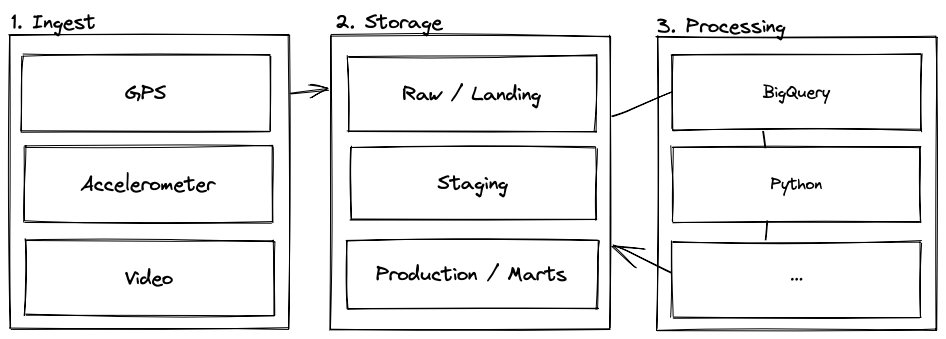
\includegraphics[width=0.95\textwidth,keepaspectratio]{images/4_data/data-platform.png}
\end{center}
\captionsetup{width=.95\textwidth}
\caption{Overview of data platform architecture.}
\label{fig:data-platform-architecture}
\end{figure}

\begin{enumerate}
\item Ingestion Layer: getting the data into the data platform. Data is manually pulled from the smartphone to a laptop. From this laptop the data is uploaded using automated scripts. Note, to ensure privacy concerns, visual data is first anonymized to remove PII data. Although this layer is not strictly within the Google Cloud Platform, it is still part of the total data platform.
\item Storage Layer: data is stored in the data platform in two services, BigQuery - a managed data warehouse solution and Cloud Storage - a generic object store. Within these two services, the data is split in three layers denoting the maturity of the data.
\begin{enumerate}
\item Raw / landing: contains the data in the form it is collected by the smartphone.
\item Staging: intermediate layer, data is processed in more useful form but not ready for consumption.
\item Production / marts: contains data ready for consumption, e.g. analyzing data and training models.
\end{enumerate}
\item Processing Layer: consumes data from the storage layer and processes it. For instance, data transformations between different areas (raw, staging, marts) or training models. Some processing steps are fully implemented with SQL and ran in BigQuery, other rely on custom Python code and are ran in Kubernetes cluster.
\end{enumerate}

In table \ref{tab:data-pipelines} all the data pipelines are listed with a description of their operation. In figure \ref{fig:data-pipelines} the pipelines are visualized (TODO: outdated). Many data pipelines are relatively straightforward and don't need further explanation than listed in the table. However, there are a few interesting processing operations further described below. The data pipelines are grouped per used data source. First we cover GPS data, then the accelerometer and finally the visual data.

% Please add the following required packages to your document preamble:
% \usepackage{booktabs}
% \usepackage{graphicx}
\begin{table}[h!]
\resizebox{\textwidth}{!}{%
\begin{tabular}{@{}p{0.25\linewidth}llp{0.6\linewidth}@{}}
\toprule
Name &
  Source &
  Destination &
  Description \\ \midrule \midrule
Ingest Accelerometer &
  \begin{tabular}[c]{@{}l@{}}Landing\\ Cloud Storage (jsonlines)\end{tabular} &
  \begin{tabular}[c]{@{}l@{}}Landing\\ BigQuery\\ \textit{raw\_accelerometer}\end{tabular} &
  Loads raw records from Cloud Storage into BigQuery table. \\ \midrule
Ingest GPS &
  \begin{tabular}[c]{@{}l@{}}Landing\\ Cloud Storage (jsonlines)\end{tabular} &
  \begin{tabular}[c]{@{}l@{}}Landing\\ BigQuery\\ \textit{raw\_gps}\end{tabular} &
  Loads raw records from Cloud Storage into BigQuery table. \\ \midrule
Ingest Wegdeel &
  \begin{tabular}[c]{@{}l@{}}External\\ Postgis\end{tabular} &
  \begin{tabular}[c]{@{}l@{}}Landing\\ BigQuery\\ \textit{raw\_wegdeel}\end{tabular} &
  Loads road sections (wegdeel) from Postgis database into BigQuery table. \\ \midrule
Ingest Frames Labels &
  \begin{tabular}[c]{@{}l@{}}Landing\\ Cloud Storage (txt)\end{tabular} &
  \begin{tabular}[c]{@{}l@{}}Landing\\ BigQuery\\ \textit{raw\_frames\_labels}\end{tabular} &
  Loads manually label annotations into BigQuery table. \\ \midrule
Ingest Label Lookup &
  \begin{tabular}[c]{@{}l@{}}Landing\\ Cloud Storage (txt)\end{tabular} &
  \begin{tabular}[c]{@{}l@{}}Landing\\ BigQuery\\ \textit{raw\_label\_lookup}\end{tabular} &
  Loads manually label definitions into BigQuery table. \\ \midrule \midrule
Determine Trips &
  \begin{tabular}[c]{@{}l@{}}Landing\\ BigQuery\\ \textit{raw\_gps}\end{tabular} &
  \begin{tabular}[c]{@{}l@{}}Staging\\ BigQuery\\ \textit{stg\_gps}, \textit{stg\_trips}\end{tabular} &
  Parses from GPS records distinct trips the car has travelled (further described below). \\ \midrule
Snap Trips to Roads &
  \begin{tabular}[c]{@{}l@{}}Staging\\ BigQuery\\ \textit{stg\_trips}\\ \\ External\\ Bing\end{tabular} &
  \begin{tabular}[c]{@{}l@{}}Staging\\ BigQuery\\ \textit{stg\_trips\_snapped}\end{tabular} &
  Snap the preprocessed GPS records to actual roads (further described below). \\ \midrule
Filter Road Sections &
  \begin{tabular}[c]{@{}l@{}}Landing\\ BigQuery\\ \textit{raw\_wegdeel}\end{tabular} &
  \begin{tabular}[c]{@{}l@{}}Staging\\ BigQuery\\ \textit{stg\_road\_section}\end{tabular} &
  Filter the road sections that are actually in use. \\ \midrule
Create Label Lookup &
  \begin{tabular}[c]{@{}l@{}}Landing\\ BigQuery\\ \textit{raw\_label\_lookup}\end{tabular} &
  \begin{tabular}[c]{@{}l@{}}Staging\\ BigQuery\\ \textit{stg\_label\_lookup}\end{tabular} &
  Converts ingested definitions to lookup table in order to join with annotated frames.\\ \midrule
Video to Frames &
  \begin{tabular}[c]{@{}l@{}}Landing\\ Cloud Storage (mov)\end{tabular} &
  \begin{tabular}[c]{@{}l@{}}Staging\\ Cloud Storage (jpg)\end{tabular} &
  Extracts separate frames from the recorded video (1 frame per second).\\ \midrule
Video to Frames Bootstrap &
  &
  &
  Spawns off separate jobs to process all video files in parallel.\\ \midrule \midrule
Link Trip Coordinates with Road Sections &
  \begin{tabular}[c]{@{}l@{}}Staging\\ BigQuery\\ \textit{stg\_trips\_snapped}\\ \\ Staging\\ BigQuery\\ \textit{stg\_road\_section}\end{tabular} &
  \begin{tabular}[c]{@{}l@{}}Production\\ BigQuery\\ \textit{mrt\_trips}\end{tabular} &
  Joins the snapped trips with the cleaned road sections from the BGT. \\ \midrule
Calculate Road Section Windows &
  \begin{tabular}[c]{@{}l@{}}Production\\ BigQuery\\ \textit{mrt\_trips}\end{tabular} &
  \begin{tabular}[c]{@{}l@{}}Production\\ BigQuery\\ \textit{mrt\_road\_section\_windows}\end{tabular} &
  Calculates timestamps (windows) when each road section was entered/exited per trip. \\ \midrule
Load Frames Labels &
  \begin{tabular}[c]{@{}l@{}}Landing\\ BigQuery\\ \textit{raw\_frames\_labels}\\ \\ Staging\\ BigQuery\\ \textit{stg\_label\_lookup}\end{tabular} &
  \begin{tabular}[c]{@{}l@{}}Production\\ BigQuery\\ \textit{mrt\_frames\_labels}\end{tabular} &
  Joins annotated frames with lookup table. \\ \midrule 
Load Frames Metadata &
  \begin{tabular}[c]{@{}l@{}}Production\\ Storage\end{tabular} &
  \begin{tabular}[c]{@{}l@{}}Production\\ BigQuery\\ \textit{mrt\_frames\_metadata}\end{tabular} &
  Creates a metadata table on the extracted frames (e.g. source video, timestamp and size). \\ \midrule 
Ingest Experiment Labels &
  \begin{tabular}[c]{@{}l@{}}External\end{tabular} &
  \begin{tabular}[c]{@{}l@{}}Production\\ BigQuery\\ \textit{mrt\_experiment\_labels}\end{tabular} &
  Ingests separate labels annotated by experiment runs into BigQuery. \\ \midrule 
Anonymize &
  \begin{tabular}[c]{@{}l@{}}Staging\\ Cloud Storage (jpg)\end{tabular} &
  \begin{tabular}[c]{@{}l@{}}Production\\ Cloud Storage (jpg)\end{tabular} &
  Automatically detect PII data and blur the detected objects.\\ \midrule
Anonymize Bootstrap &
  &
  &
  Spawns off separate jobs to process all source files in parallel.\\ \bottomrule
\end{tabular}%
}
\caption{Overview of all the different data pipelines.}
\label{tab:data-pipelines}
\end{table}

\begin{figure}[h!]
\begin{center}
\makebox[\textwidth][c]{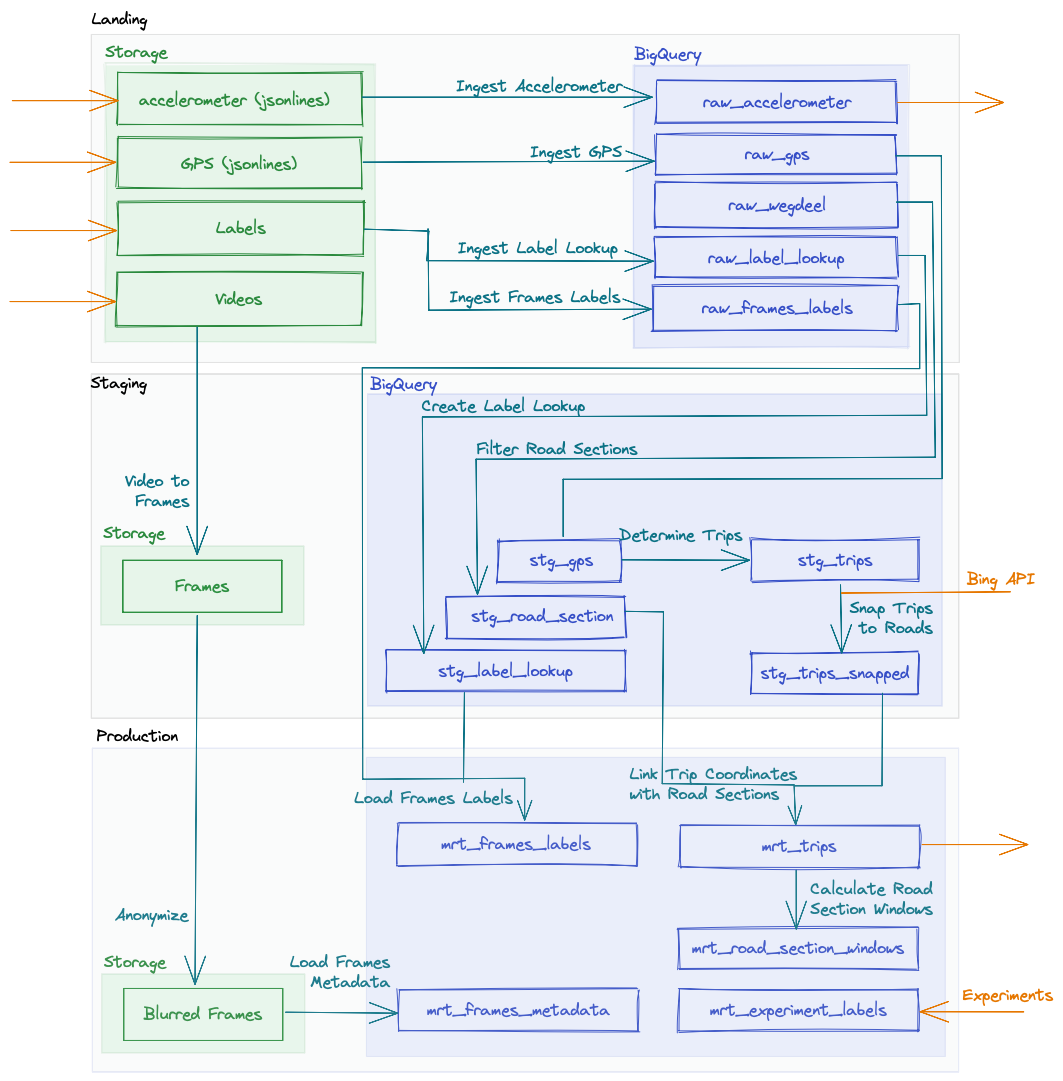
\includegraphics[width=1.2\textwidth,keepaspectratio]{images/4_data/data-pipelines.png}}
\end{center}
\caption{Visual overview of the various Data Pipelines.}
\label{fig:data-pipelines}
\end{figure}


\subsection{GPS Data}
GPS data describes the location of the vehicle in coordinates. Specifically the coordinates are recorded in latitude and longitude information as notated in WGS84 standard. The data is sampled at 1 Hz. GPS data is further processed to find distinctive trips and to calculate speed and heading information of  the travelling vehicle.


\subsubsection{Determine Trips}
The GPS sensor records the location of the vehicle. After ingestion, this data is stored in raw form on Google Cloud Storage (GCS). The format of the data is stored as json lines. This is a file format where each line in the file is a single json document. Within this document the location of the vehicle is recorded with the respective time. After the data is ingested in BigQuery, the GPS data is deduplicated and distinctive trips are detected with the following algorithm. Each trip as an unique identifier, with these distinctive trips it is easier to fuse different sources i.e. querying the accelerometer data from a specific trip.

\begin{enumerate}
\item Deduplication: the GPS sensor always records location data. If the car is standing still (e.g. traffic light), the data is still recorded, resulting in duplicate records. The first step is to deduplicate the data. This is done by selecting the first record for each unique location in subsequent time series. 
\item Delta calculation: between each subsequent record the difference between time and distance is calculated.
\item Split trips: trips are detected from the consecutively records by finding records where the vehicle is stationary longer than 120 seconds. This commonly known as dwell time, and 120 seconds is often used in literature \cite{Wolf2001}.
\item Reset trips: for each first record of a trip, the delta time and distance is reset to zero.
\item Cleanup trips: to cleanup invalid data, only trips are selected with more than 5 records of data and with at least 500 meters travelled in total.
\end{enumerate}


\begin{figure}[H]
  \centering
  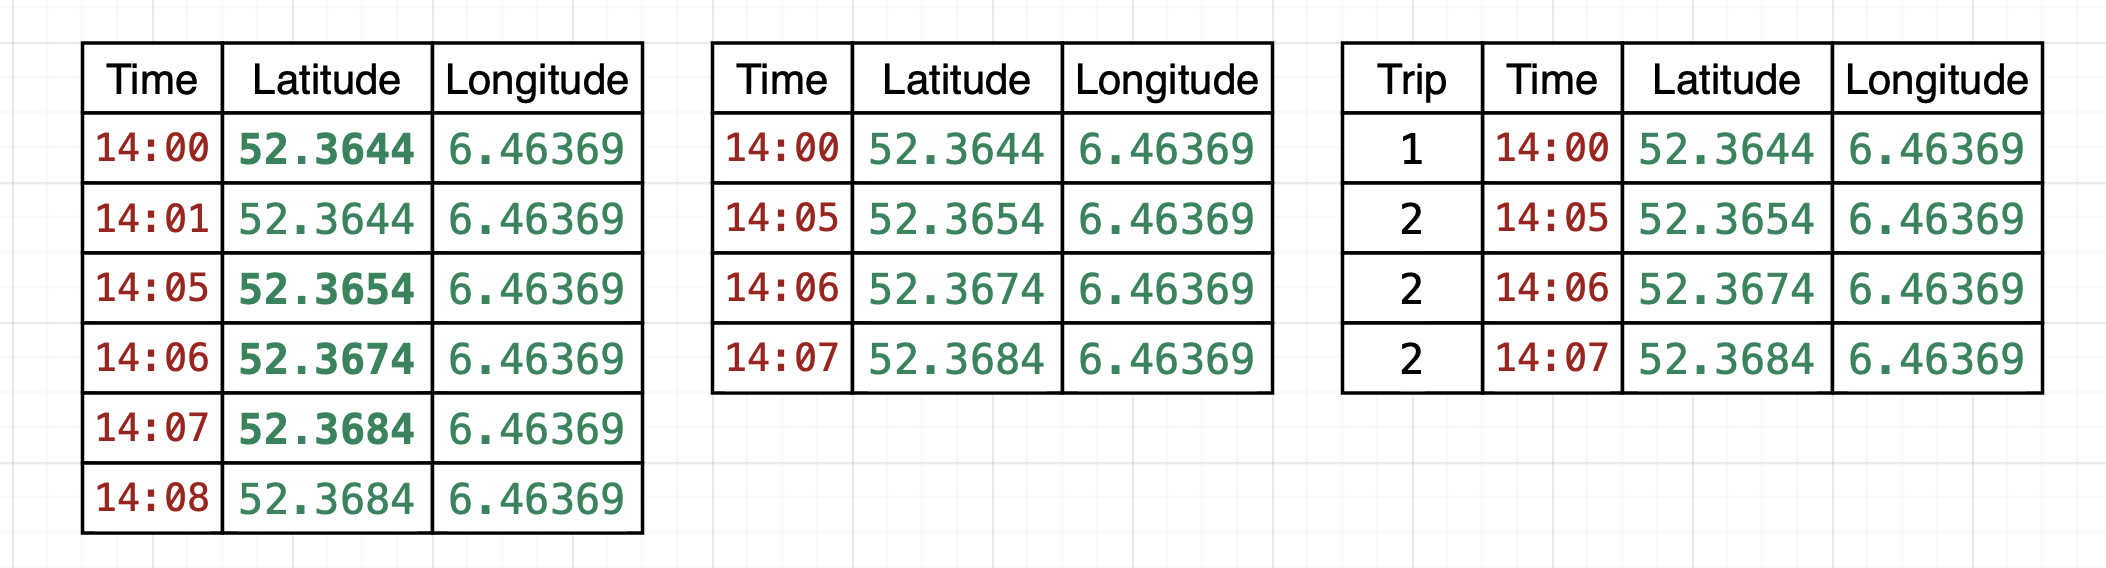
\includegraphics[width=0.95\linewidth]{images/4_data/trip-detection.png}
  \captionsetup{width=.95\textwidth}
  \caption{Example of trip deduction algorithm. Left shows original data, center shows after deduplicating based on the location, right shows the resulting trips.}
  \label{fig:test2}
\end{figure}




\subsubsection{Snap Trips to Roads}
GPS data is generally regarded as noisy. The accuracy of the sensor varies over time. Resulting that some coordinates are aligned on roads, while other samples are outside the road. See also figure \ref{fig:snap-trips}. This becomes an issue when we further process the data. In our case, we want to join GPS data with ground truth data for the roads. This allows to compare data from distinctive trips on the same roads, or to find build information of the roads (further described below). To cleanup this data, GPS coordinates are snapped to actual roads. The anchoring of the GPS coordinates is done with an external service. In this specific case "Snap Points to Roads" from Bing Maps \cite{Snap-Points-to-Roads} is used, but there are other APIs that perform this service.


\begin{figure}[H]
\begin{center}
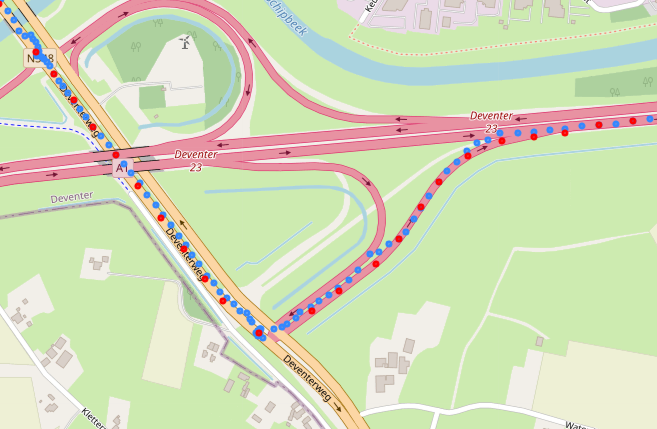
\includegraphics[width=.95\textwidth,keepaspectratio]{images/4_data/snap-trips.png}
\end{center}
\captionsetup{width=.95\textwidth}
\caption{Display of snapping coordinates to roads. The blue dots are the measured GPS coordinates, and the red dots are the inferred coordinates by external service. Note that some of the blue dots are on the wrong lane or beside any roads.}
\label{fig:snap-trips}
\end{figure}

\subsubsection{Link Trip Coordinates with Road Sections}
\textit{Basisregistratie Grootschalige Topografie} (BGT) is registry in the Netherlands of "large-scale objects in the public space". This registry marks all locations and their bounding area (in coordinates) of large-scale objects such as roads, buildings and territory. The BGT is regulated by law, and is mandatory for governments to use and maintain while operating in the public space \cite{BGT}. The BGT also includes roads as \textit{road sections}. The size of a section varies to a single street bump in a town, to several hundred meters of highway. Road sections are annotated with various types of attributes, of which one is promising for this thesis. That is the material of the road: concrete, asphalt or brick. The road snapped GPS coordinates are joined to the respective road sections from the BGT.


\subsubsection{Calculate Road Section Windows}
Road sections cover a geographical area, and therefore are likely to contain multiple GPS records. Sensor data (visual and accelerometer) can only be linked with GPS through their respective timestamps. To link these data sources each road section it is calculated when that section was entered and exited. This is referred as the \textit{road section window}.

\subsection{Accelerometer Data}
Accelerometer measures acceleration, the change of velocity over time. In the smartphone the sensor measures acceleration in three axis: longitudinal (X), lateral (Y) and vertical (Z) axes. The output is in G-forces, where $1 G = 9.81m/s^2$. In stationary position, the accelerometer always measures 1G on the vertical axis due gravitational pull of the earth. Acceleration data describes the vibrations of the vehicle. However, before the data can be used, it needs to be pre-processed. Of which the most important is that the orientation of the sensor needs to be aligned with that of the vehicle. All processing steps are described down below.


\subsubsection{Re-sampling}
Re-sampling the data ensures a constant sampling frequency. This is necessary for further signal processing operations such as calculating FFT or filtering noise. This step was required when collecting data with the AutoPi (the first method). From data analysis it appeared that the AutoPi had variations in the sampling rate. With the new data collection method, the smartphone collects the accelerometer data more consistently. To ensure a consistent sampling frequency, this processing step is still applied, even for the newer collection method.

Re-sampling of the data is done by fitting a B-spline curve for all the known samples. From this spline, the data points are uniformly sampled at the expected frequency. The effect of re-sampling is shown in figure \ref{fig:accelerometer-resampling}. Note that the example in this figure was of data collected with the AutoPi. For data from the smartphone the effect is less noticable. The top blue graph shows the raw readings from the accelerometer. The bottom red graph shows the resulting data after re-sampling. Notice that the interval between readings of the top graph is variable, whereas the bottom is uniformly spaced. This approach of resampling also been used in \cite{Wu2020}.

\begin{figure}[H]
\begin{center}
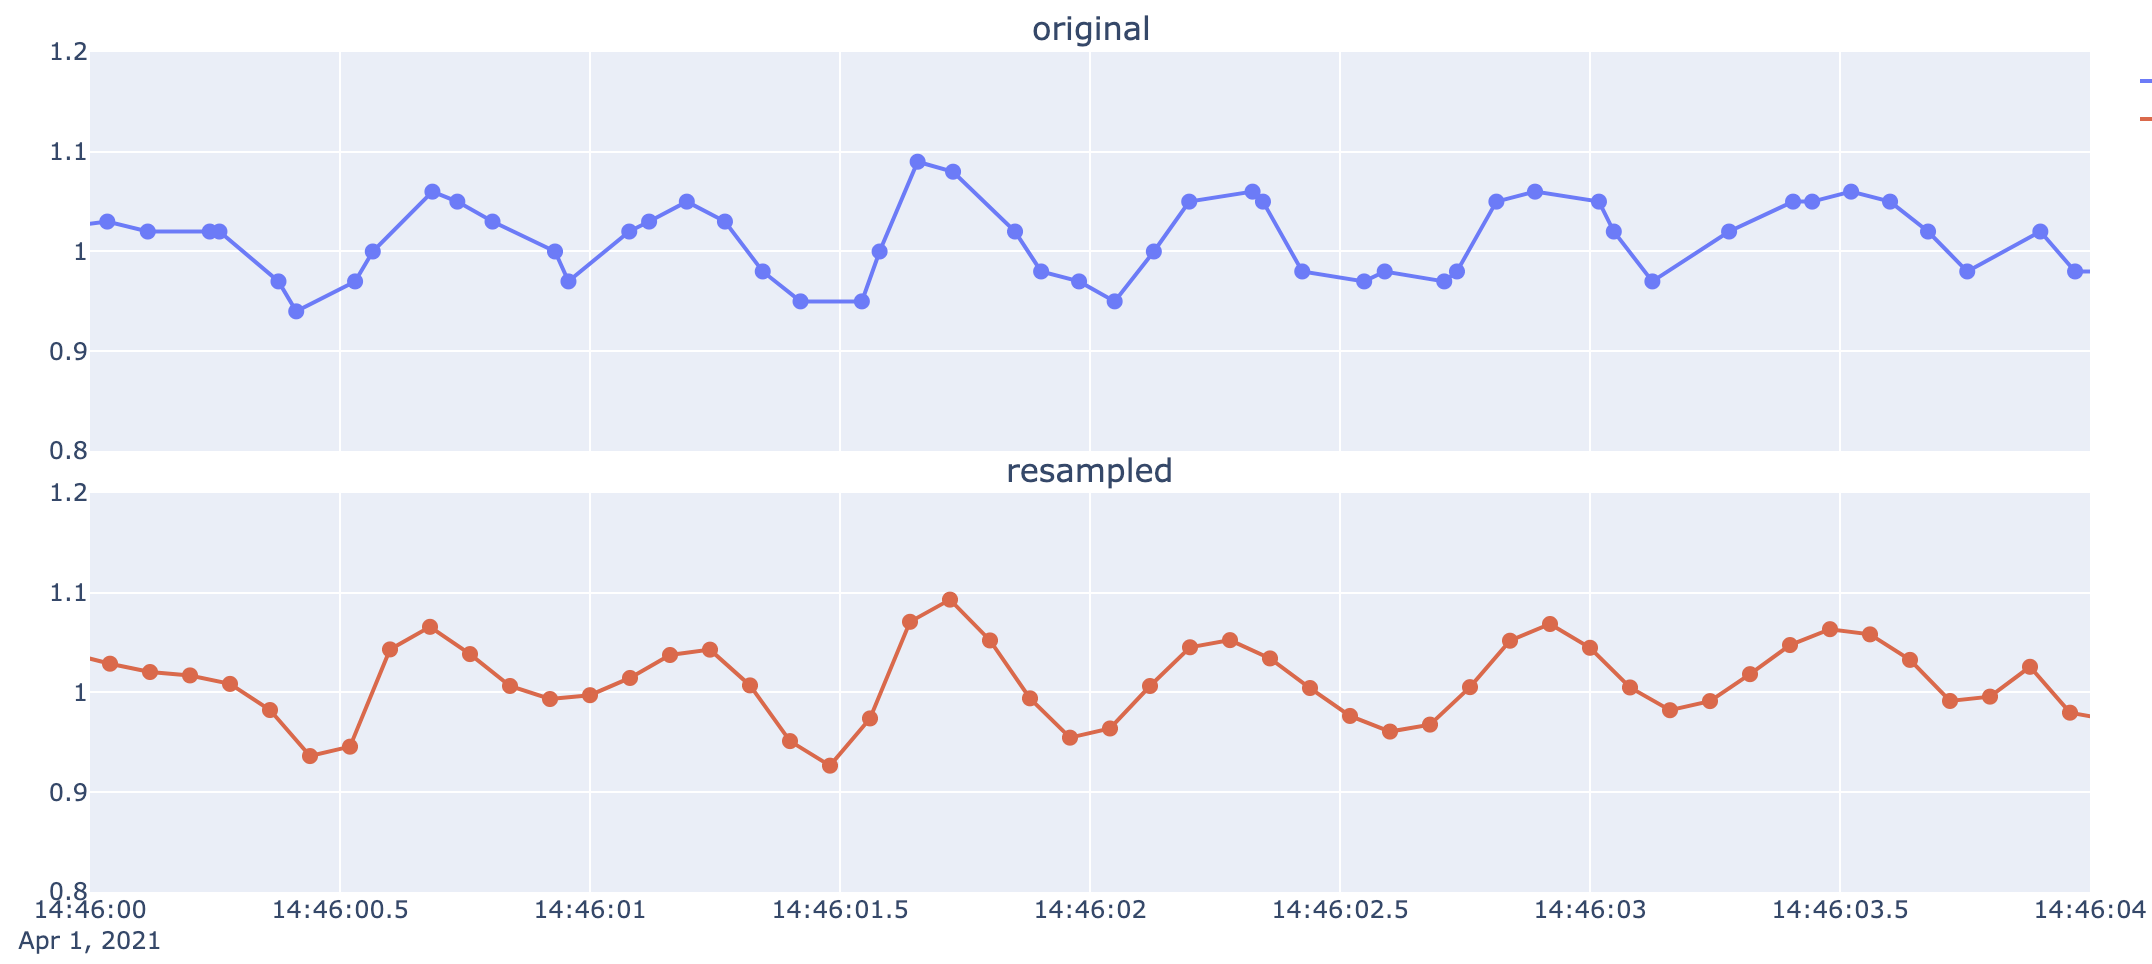
\includegraphics[width=.95\textwidth,keepaspectratio]{images/4_data/accelerometer-resampling.png}
\end{center}
\captionsetup{width=.95\textwidth}
\caption{Top graph displays the raw data from the accelerometer. Bottom graph displays the accelerometer data after re-sampling. Note this example is made on data from AutoPi, where the effect is more prominent.}
\label{fig:accelerometer-resampling}
\end{figure}


\subsubsection{Realignment}
The coordinate system of the accelerometer may not coincide with that of the vehicle. Meaning, when the vehicle drives over a bump it is expected to see a acceleration in vertical axes. However, when it is not aligned, the acceleration is shown on a different axes or as a product of axes. There are two causes for this misalignment. First, we don't know how the sensor is oriented in the smartphone, making it hard to align it correctly.  As the same smartphone also needs to record the road, aligning it in such way is futile regardless. Secondly, we can't expect to place the smartphone perfectly consistent at the same angle every time in the holder. Before any of the data can be analyzed, the coordinate system of the accelerometer must be aligned with that of the vehicle. To fix this issue, a process was developed to automatically align the coordinate systems. Making it also possible to generalize collection of data to any vehicle and accelerometer sensor. This process has been inspired by \cite{accelerometer_alignment} and is also applied in \cite{Wu2020}. 

The process consists of two steps. First, the coordinate system is aligned on the vertical Z-axes using a rotation matrix $R_z$. Subsequently, the horizontal plane is aligned using a rotation matrix $R_x$. Calculating these rotation matrices is done by measuring the accelerometer sensor $a_s$when a known force is exerted on the vehicle, $a_v$. Using Euler angles we can calculate the rotation matrix to align the force $a_s$ to that of the known force $a_v$. In the figure \ref{fig:align-vectors} the two-step method is visually presented.


\begin{figure}[H]
\begin{center}
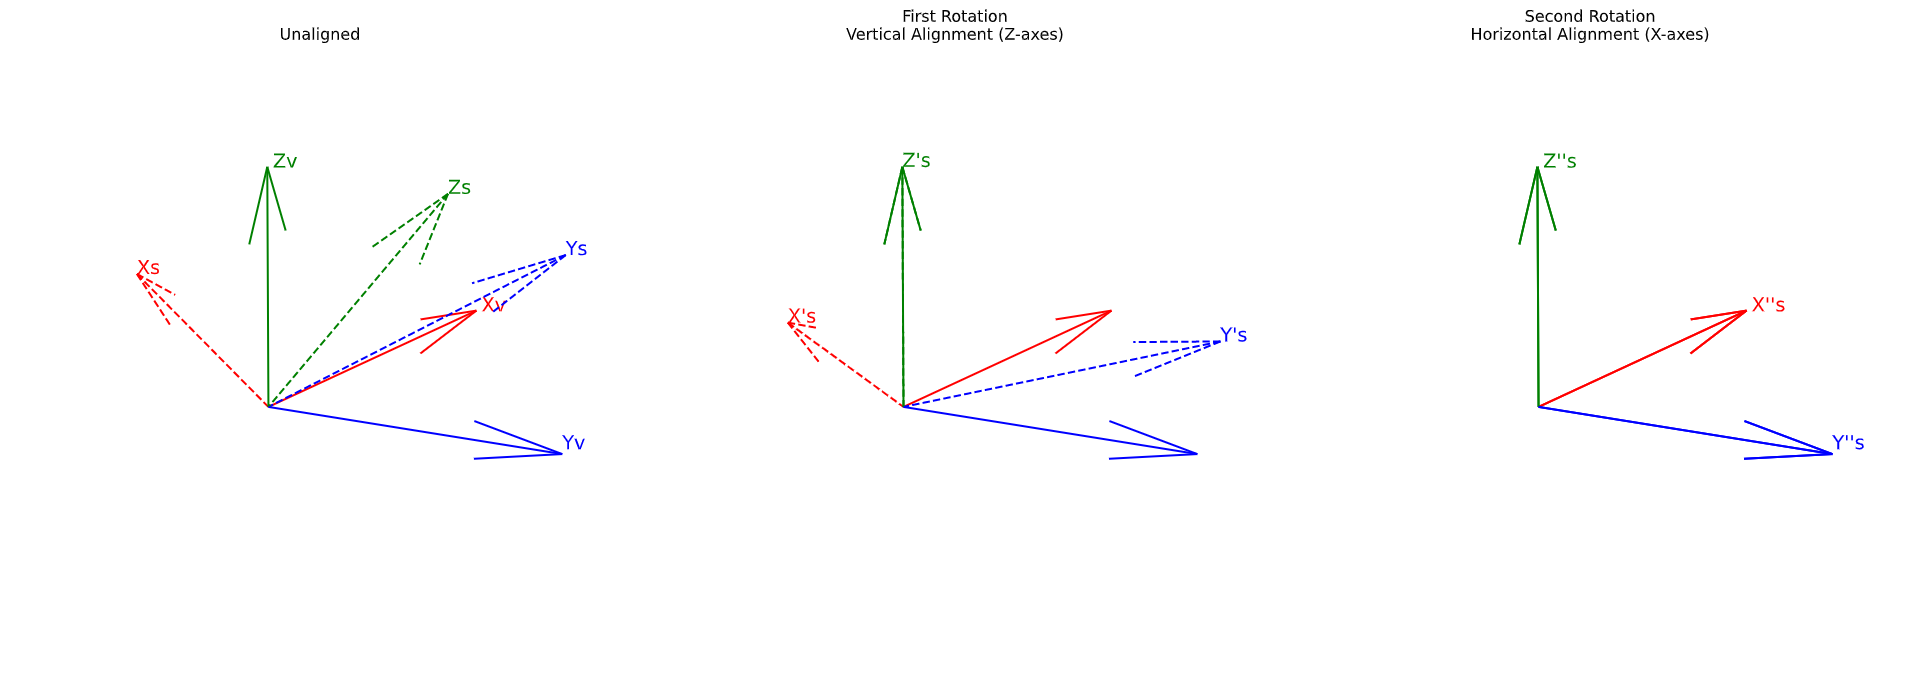
\includegraphics[width=0.95\textwidth,keepaspectratio]{images/4_data/accelerometer-alignment.png}
\end{center}
\captionsetup{width=.95\textwidth}
\caption{Figure displaying the process of aligning the axes. Zv is the Z-axes for the vehicle, Zs is the Z-axes for the sensor. Left: shows the original, unaligned situation. Middle: shows the situation after aligning the Z-axes. Right: shows situation after aligning the X-axes.}
\label{fig:align-vectors}
\end{figure}



For the first step, aligning the vertical Z-axes, the known force is the gravity of the earth. When the vehicle is stationary, the expected force is $a_v = (0, 0, 1G)$. Stationary points are found by querying the GPS data when the car is not moving. Ideally, only accelerometer data is used when the vehicle is on a level surface. As we don't have access to this information, we rely on taking the average of many samples, as it can be assumed that on average the vehicle is mostly stationary on a flat surfaces. This assumption seems plausible in the Netherlands, where the country is largely flat. See also section \ref{section:stationary-points} for detailed discussion. The rotation matrix $R_z$ is calculated to align vector $a_s$ onto vector $a_v$ as follows \cite{rotation_matrix}. 

\begin{flalign*} 
\text{Let } v &= a_s \times a_v \\
\text{Let } c &= a_s \cdot a_v \\
\text{Let } skew &=
\begin{bmatrix} 0 & -v_3 & v_2 \\ v_3 & 0 & -v_1 \\ -v_2 & v_1 & 0 \end{bmatrix} \\
R_z &= I + skew + skew^2 \frac{1}{1 + c}
\end{flalign*}

The second step is to align the coordinates system in the longitudinal X-axes. Again, we take readings of the accelerometer when a certain force is expected. In this case when the car is braking, the expected acceleration is $a_v = (-x, 0, 1G)$, where $x$ depends on the deceleration of the vehicle. Braking windows are selected based on the derived speed from the GPS coordinates. As the vertical axes is already aligned, we need to calculate a two dimensional rotation matrix $R_x$ to align vector $a'_s$ onto vector $a_v$ in the longitudinal X-axes. $a'_s$ refers to the measured acceleration after applying the rotation.

\begin{flalign*} 
\sin \theta &= a'_s \times a_v \\
\cos \theta &= a'_s \cdot a_v \\
R_x &= \begin{bmatrix} \cos \theta & -\sin \theta & 0 \\ \sin \ \theta & \cos \theta & 0 \\ 0 & 0 & 1 \end{bmatrix} \\
\end{flalign*}




\subsubsection{Noise filtering}
Accelerometer data is prone to noise. As is common with signal processing, data is first passed through a filter to obtain a clearer signal. Noise in the signal comes from vibrations generated by vehicle. Additionally, from research it is stated that specific events causes noise such as braking, acceleration and steering. Existing research uses a variety of different filter configurations to clean the data. Some apply a low-pass Butterworth filter \cite{Gupta2020}, whereas other researches use a high-pass Butterworth filter \cite{Wu2020, Janani2020}. Refer back to section \ref{sec:butterworth-filter} for detailed explication of Butterworth filter. Due the different usages, we assume that it differs per application and approach it as a possible tuning parameter.

In figure \ref{fig:filter}, various configurations of a 5th-order Butterworth filter are displayed. At the top left (blue) is the original signal while driving over a manhole. The other graphs shows the resulting signal after applying a specific configuration. For instance, the middle right (orange) is after passing the data through a high pass filter with cut-off at 2 Hz. Meaning that all frequencies below 2 Hz are filtered out. As this signal seems most clean, we use this configuration as an initial starting point. In future, other types of configurations can be applied to optimize performance. 


\begin{figure}[H]
\begin{center}
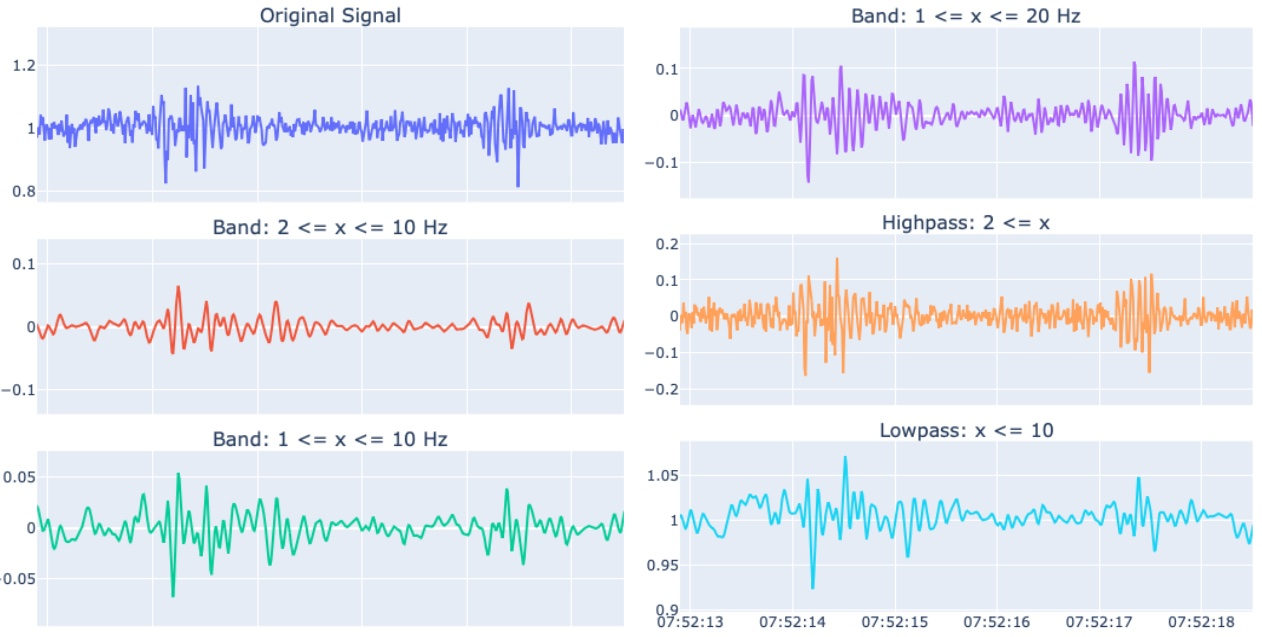
\includegraphics[width=0.95\textwidth,keepaspectratio]{images/4_data/filter-example.jpg}
\end{center}
\captionsetup{width=.95\textwidth}
\caption{Figure displaying various graphs after applying a 5th-order Butterworth filter to the accelerometer signal on the vertical Z-axis. The event shown here is when the vehicle drives over a manhole.}
\label{fig:filter}
\end{figure}




\subsection{Visual Data}
\label{sec:visual-data}

As previously mentioned the road suface is recorded with an Apple iPhone 12 Mini. The data is recorded at resolution of 1280 x 720 at 30 frames per second (FPS). The phone is located in a generic  phone holder attached to the windshield. As can be seen in the setup figure \ref{fig:smartphone-collector}, the camera angle is parallel to that of the road surface. This means that the camera also records other data than the road such as other vehicles, the sky and other surroundings. Below described are the processing steps for the visual data. Before the visual data is uploaded to the data platform it is anonymized. Therefor these processing steps are ran at local machine, as opposed to the earlier described steps.


\subsubsection{Video to Frames}
All visual data processing operations operate on single frames instead of video files. Therefore, the first step is to extract the distinctive frames from the video. The open-source tool FFmpeg \cite{ffmpeg} is used to convert the video to the frames. The frames are linked with their respective timestamps as recorded by the data collection app.


\subsubsection{Anonymization}
Although not intentional, the camera may record other cars, persons and other PII data. To safeguard any privacy concerns, the data is anonymized. This is done by blurring PII data from the individual frames. Detection of PII data happens with pre-trained object detector YOLOv5 model \cite{Jocher2021}. This model is trained on COCO dataset, and thus is capable of detecting various classes among which are: [person, bicycle, car, motorcycle, airplane, bus, train, truck, boat. After the frames are anonymized, the frames are uploaded to the data platform. 


\subsubsection{Optical Flow}
Visual and accelerometer data can be synchronized when the same events are present in both modalities. Dense optical flow estimates the acceleration between two frames. Using optical flow it is possible align visual and accelerometer data. This has also been further described in section \ref{section:synchronization}. 

For each of the extracted frames, the optical flow is calculated. This is done with the Farneback algorithm\cite{Farnebäck2003}. The average of output is taken which results in a 2D vector field, describing the full motion of the frame in horizontal X- and vertical Y-axis. In figure \label{fig:optical-flow} the results are shown. At the top the input frame is shown in raw form, and after calculating the optical flow. The bottom graphs compares the full vertical optical flow with that of measured accelerometer data. Although it is not visible in on this graph, there exists a small delay between the modalities due time synchronization. Referred to as $\tau_{capture}$. Synchronization of these modalities is tackled in section \ref{sec:capture-time-synchronization}.

\begin{figure}[H]
\centering
\subfloat{{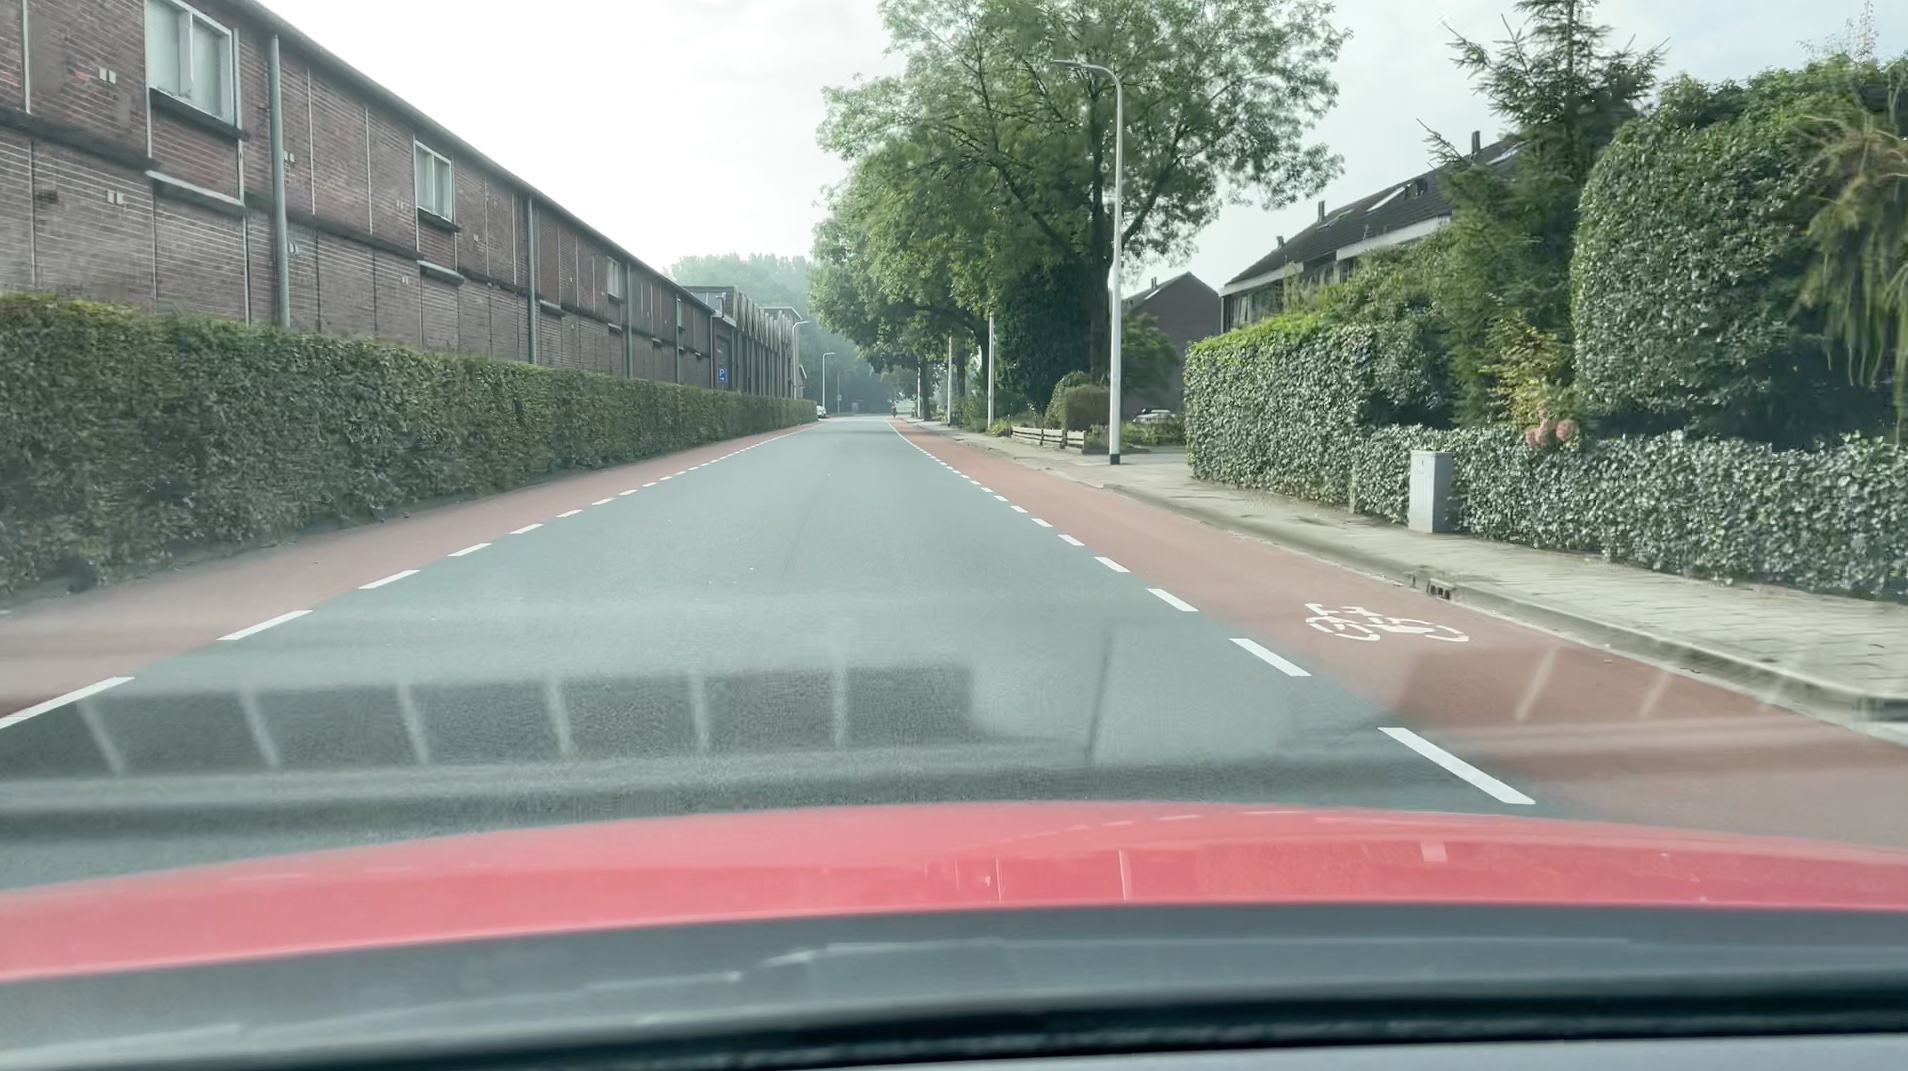
\includegraphics[width=0.45\textwidth,keepaspectratio]{images/4_data/original.jpg} }}%
\quad
\subfloat{{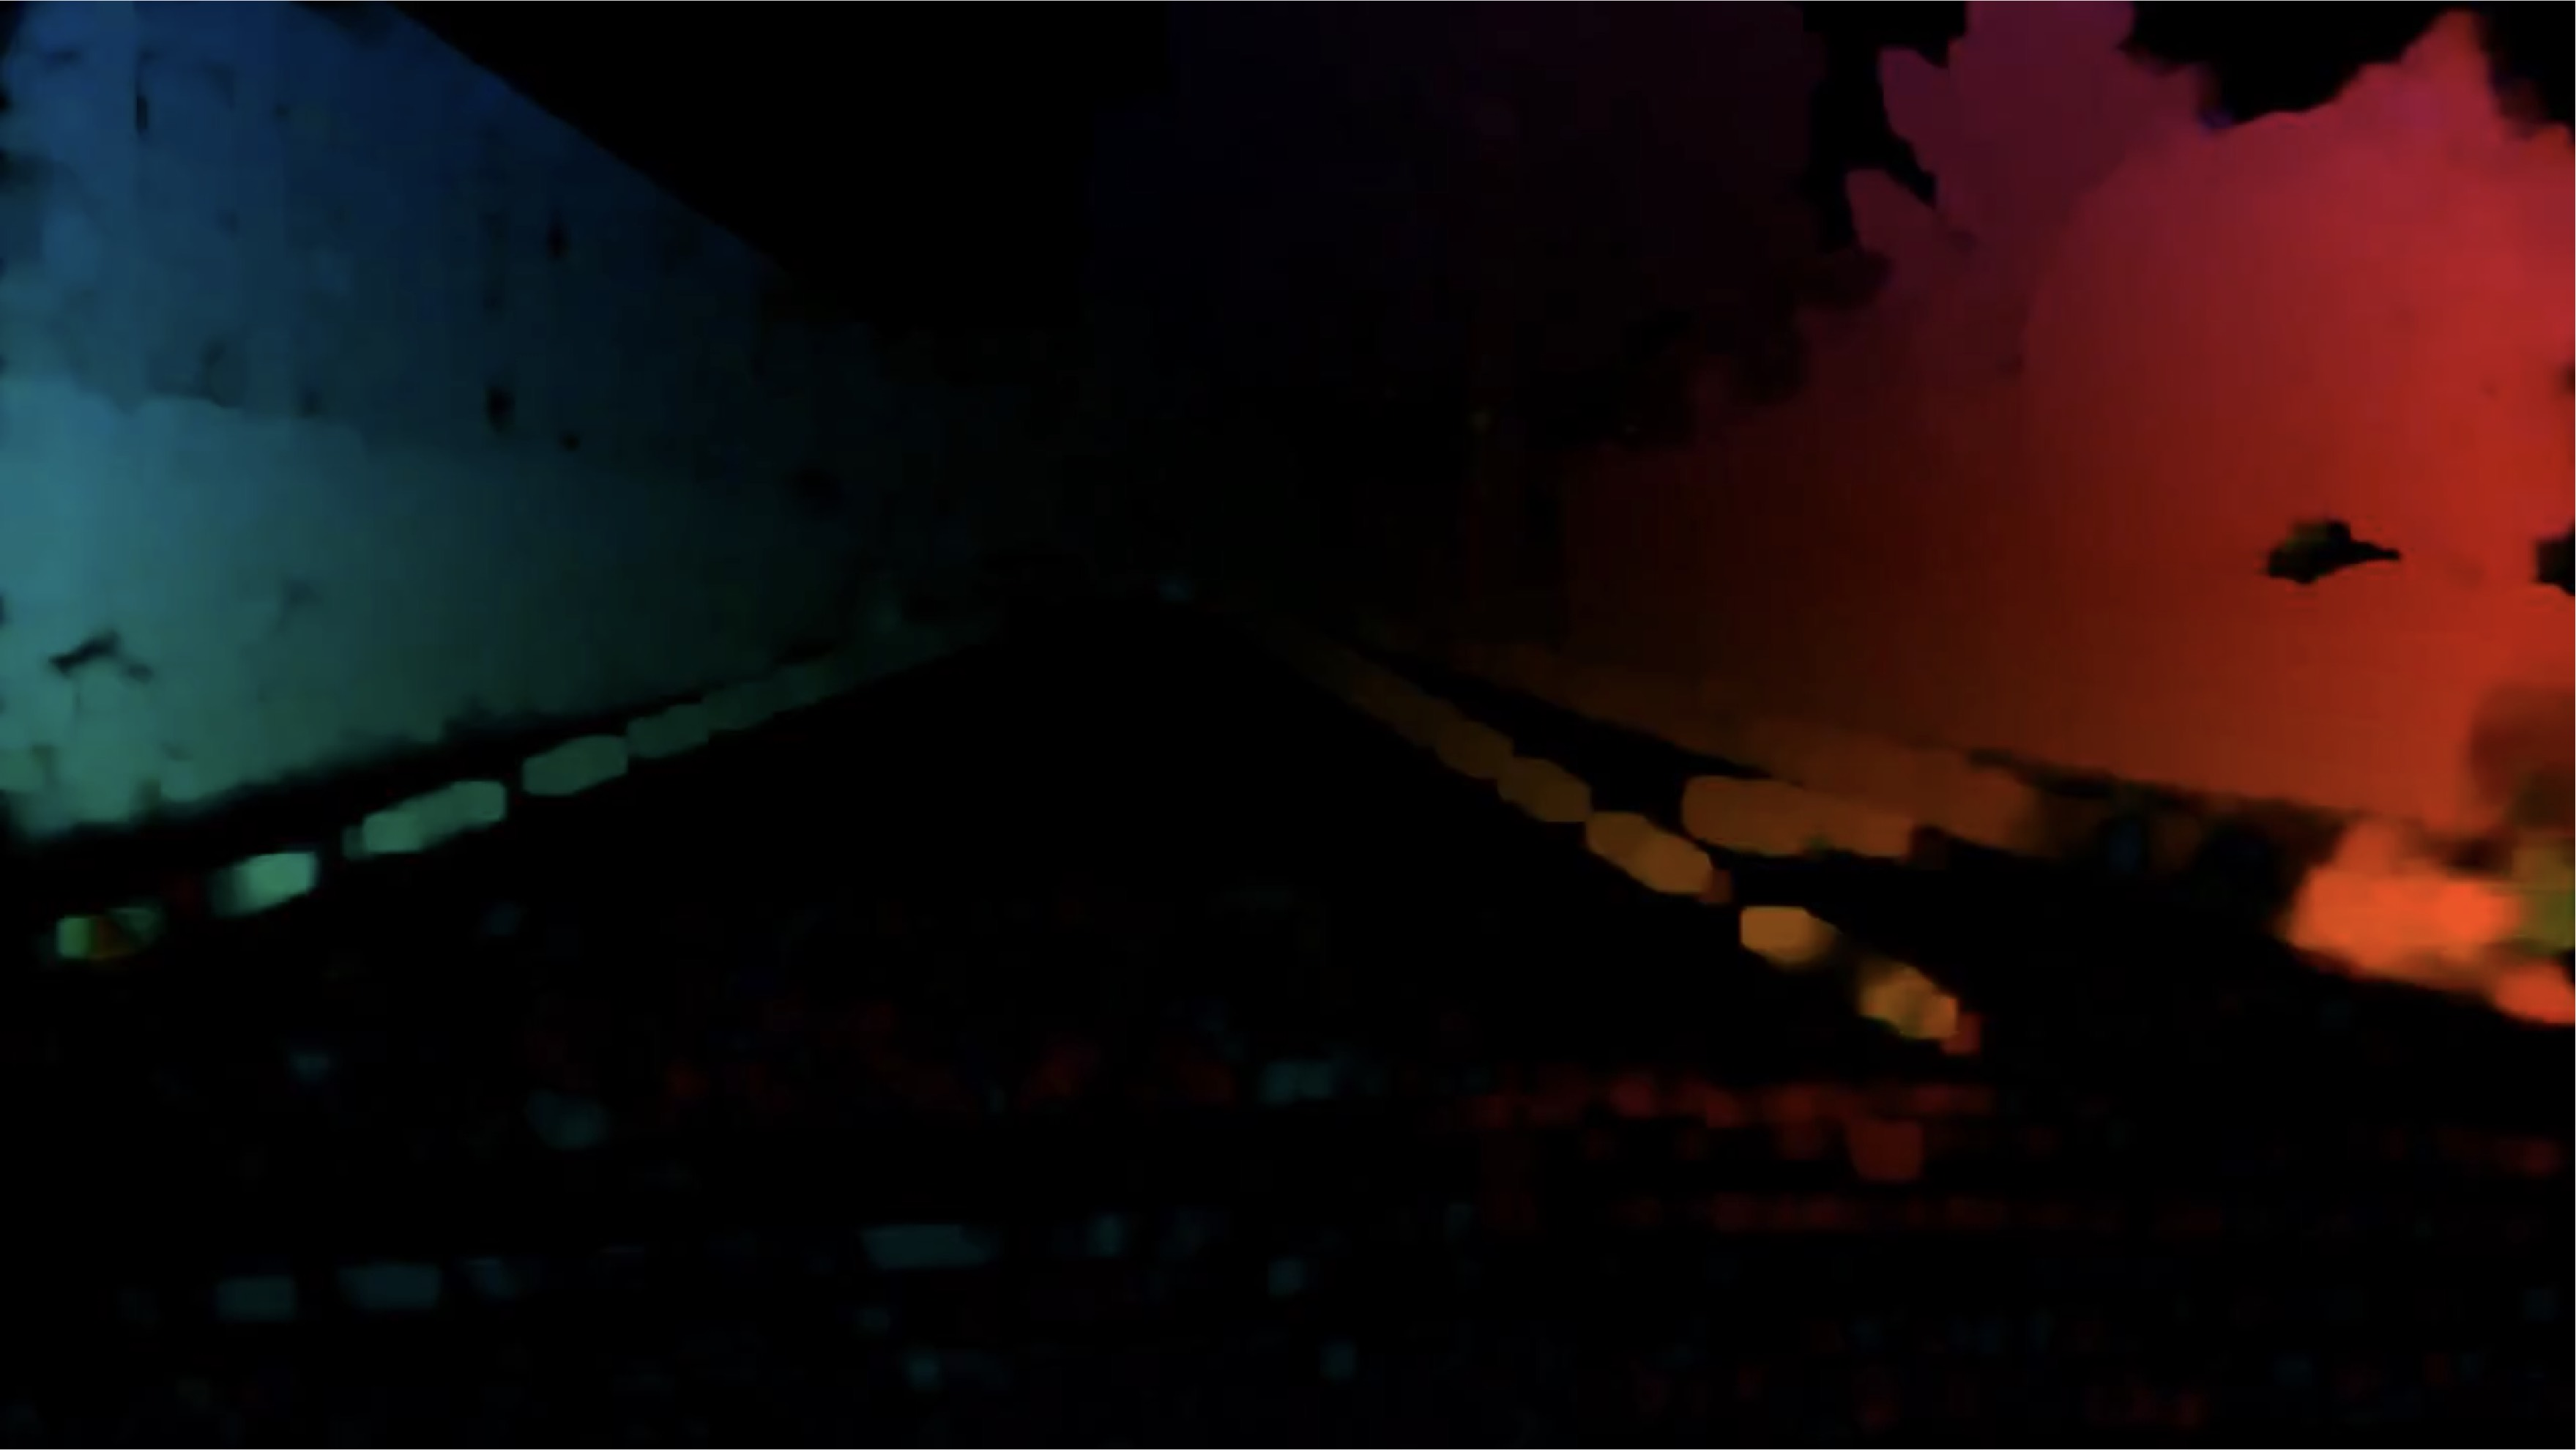
\includegraphics[width=0.45\textwidth,keepaspectratio]{images/4_data/optical-flow.jpg} }}%
\label{fig:optical-flow}
\end{figure}

\begin{figure}[H]
\centering
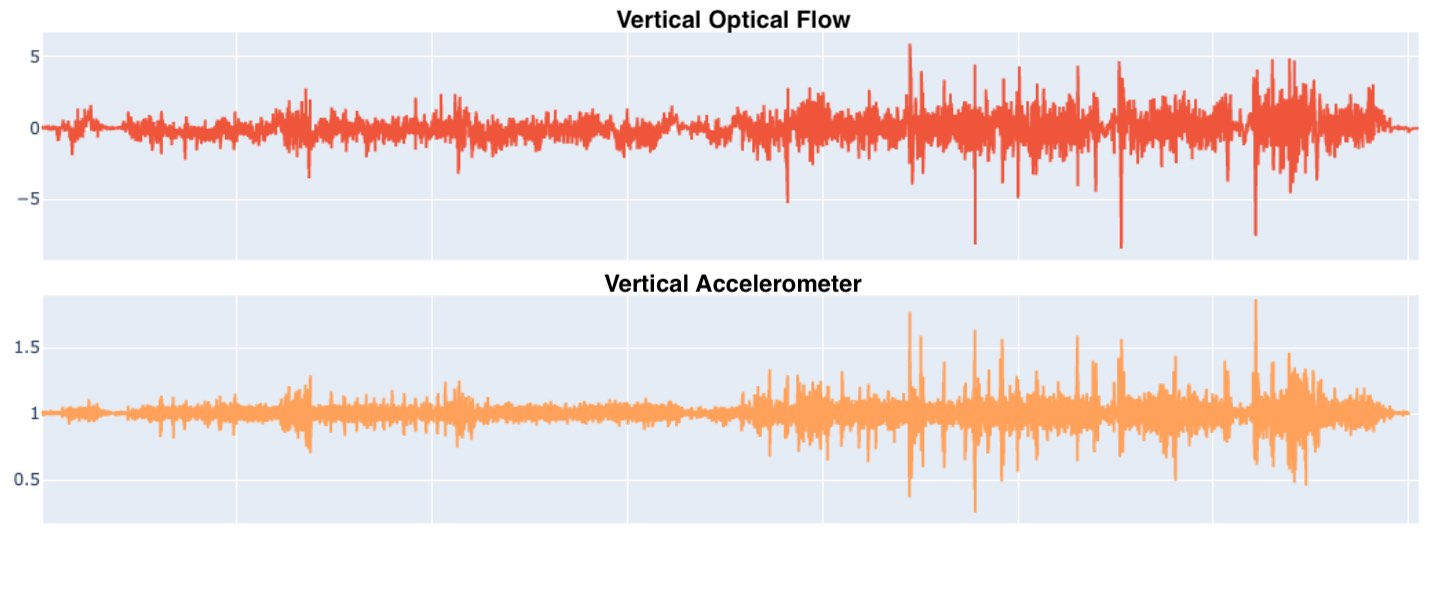
\includegraphics[width=0.95\textwidth,keepaspectratio]{images/4_data/optical-flow-graph.jpg}
\end{figure}




 
